% chap4.tex 


\chapter{Visibility guided multimodal volume visualization }\label{chap:errors}


\section{Motivation }

It is often desirable to visualize multimodal data by rendering the multiple volumes into one image. The general approach to this visualization is to fuse the multiple datasets based on their weighted intensity values. For example, CT is usually used to give us contextual information, to show anatomical relationship between pathological tissue (highlighted with PET data) and other non-effective regions. However with this approach, the intensity of the target area is often similar to that of neighbourhood resulting in lack of focus and clarity of sections of interest.  Another approach when intensities are similar, is to manually segment out a part, and define a separate transfer function for highlighting the target area. Such manual tasks are tedious and error-prone.  

\section{Context+Focus Visualization For Multimodal Volume}

The advantage of using additional modalities is that they provide complementary or supplementary information. However, handling of multiple sources for a structure, and generating a single image from them, is quite challenging.  
 
The notion of visibility, as discussed in the previous chapter, helps us to summarize distribution for visibility a structure of interest from a given viewpoint. For example PET and CT dataset, PET data acts as the ROI we need to focus and CT data gives us the context. The techniques discussed in the previous chapter can used to modulate CT data opacities to obtain "focus+context" visualization. 

\section{Local Visibility Histogram}

One technical challenge that lies in multimodal dataset visualization is in ROI definition. One way would be set up a ROI around the structure of interest manually by identifying some key boundary points. If the structure is complex, user needs to define a larger number of boundary points around the ROI, which is time-consuming and error-prone. One solution to this problem is to define a sphere or bounding box covering the ROI, as shown in figure 4.1. This solution is difficult to adopt, when the structure is complex, scattered or noisy. 


\begin{figure}[!h]
\centering
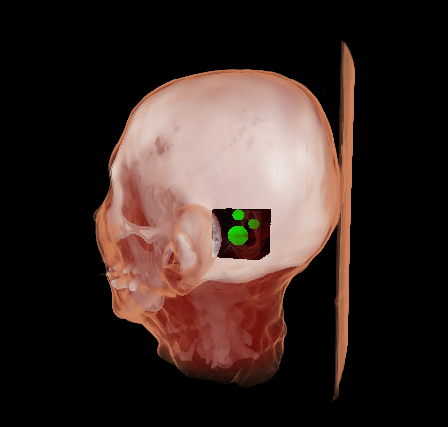
\includegraphics[width=350pt]{Images/Vol-ROI.png}
\caption{\label{fig:ray_cast1.jpg} ROI bounded by a volume.}
\end{figure}

One approach to increase visibility of ROI is to make occluding materials completely transparent, but this completely loses all the context information. Hence, for those rays hitting the ROI, local histograms is computed for each ray, as shown in figure 4.2. Rest of the rays cast into the volume are used to compute the global histogram. Using this, the user will now be able to manipulate the area of ROI, and control the visibility of this area. Upon varying the view direction local histogram is recalucated. 


\begin{figure}[!h]
\centering
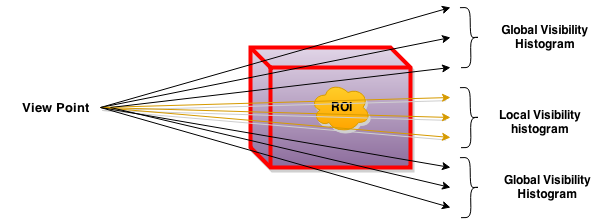
\includegraphics[width=300pt]{Images/pet-ct-roi.png}
\caption{\label{fig:ray_cast1.jpg} Global histogram and local histogram.}
\end{figure}
 

Once visibility histogram is known, opacity of samples in the ROI are adjusted using the formula 4.1.

\begin{equation} 
A^{'}(x) \; = \; A(x) \; ( \; 1 \; - \; VH(X) \; )^{e} 
\end{equation}

where, A($x$) and A$^{'}(x)$ are the old and new opacity mappings for intensity $x$. VH($x$) is the visibility associated with that intensity in the visibility histogram. $e$ is the exponent that defines the strength of such a mapping, as illustrated in the figure 4.3.

From equation 4.1, when VH($x$) is high(ie., it is more visible) it is likely to be made more transparent. When VH(x) is low, these samples do not occlude much and are retained to provide context. This helps in keeping context clear which increasing the focus. 


\begin{figure}[ht]
\centering
%\begin{minipage}[b]{0.45\linewidth}
e = 0    \hspace{140pt}      e = 1 \\
\vspace{3pt}
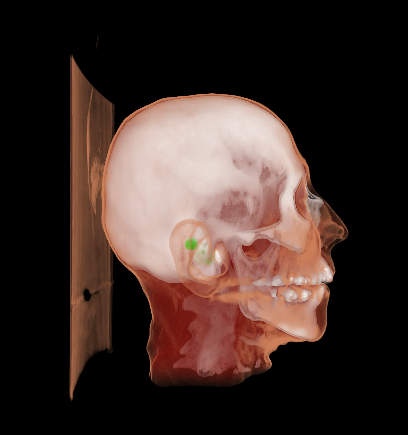
\includegraphics[width=150pt,height=150pt]{Images/i=0.png}
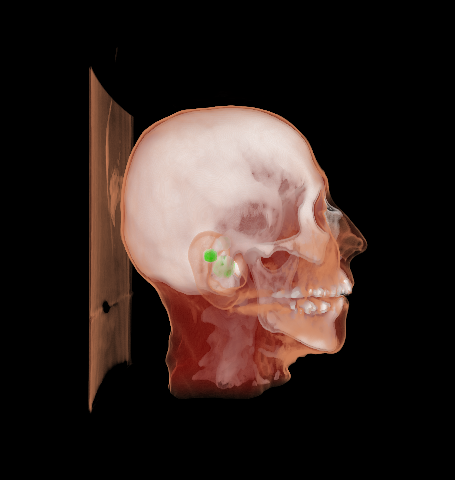
\includegraphics[width=150pt,height=150pt]{Images/i=1.png}\\
e = 3    \hspace{140pt}      e = 10 \\
\vspace{3pt}
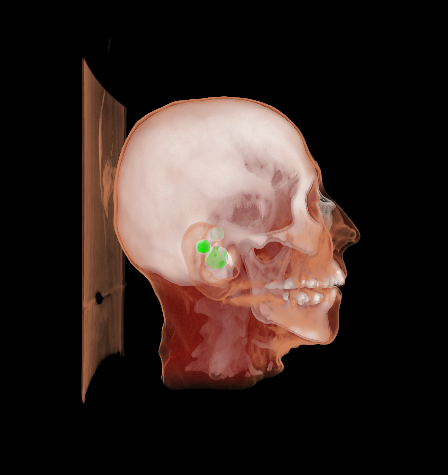
\includegraphics[width=150pt,height=150pt]{Images/i=3.png}
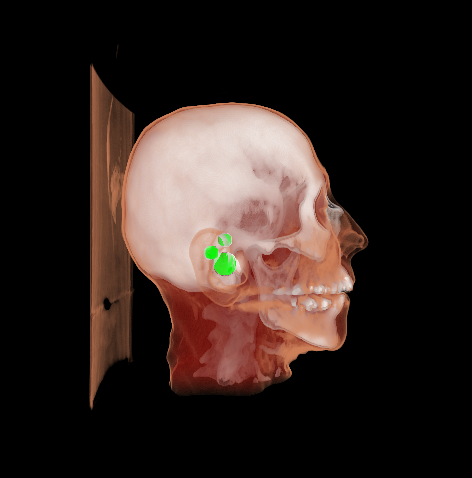
\includegraphics[width=150pt,height=150pt]{Images/i=10.png}
\caption{Effects of visibility-weighted adjustment $e$. }
\end{figure}



